\newpage

\chapter{Building a web application interfacing the derivation engines.}

The following section focuses on providing an overview of the solution implemented. It also explores various design and implementation choices made. Lastly, an evaluation of the current implementation and its alternatives is explored.

\section{Overview of the Solution.}

The web application's architecture is based on a 3-tier system that includes three distinct parts that make up the application. These parts of the application communicate between each other to provide the user with the final desired outcome. 	The system is made up from the Client, Server and Derivation Engines. The Server acts as a coordinator between the Client and the Derivation Engines. Users interact with the client side of the application which then communicates with the Server. The Server then process the request from the user and submits it to the eligible Derivation Engine. Once the derivation is complete the Server process the solution and sends it back to the client as illustrated in [TODO].

\subsection{Client}

The Client part of the application is the user's gateway to the argumentation derivation engines. It provides the user with a GUI providing both the means required to submit an argumentation framework and  the tools required to view the derivation tree received. It also allows the user to specify which engine and what semantics are to be used.

It was built using tools such ASP.Net and Javascript. ASP.Net, along with HTML was used to create the web pages the user can interact with. Javascript and the D3.js library where used to provide a useful visualisation of the outcome to the user in the form of a derivation tree.

\subsection{Server}

The Server part acts as a coordinator between the Client and the Derivation Engines. Within the Server the input from the Client is processed and prepared to be given to the necessary derivation engine to be analysed. The Server part carries out the following functionality:

\begin{itemize}

\item Analyses the parameters from the user and selects the correct derivation engine and semantics.
\item Parses the user's input, processes it and generates the relative input for the derivation engine.
\item Grounds the framework provided by the user over the domain specified.
\item Parses and analyses the output from the derivation engine and builds a JSON string that is passed to the client to build the derivation tree visualisation.

\end{itemize}

\subsection{Derivation Engines}

The Derivation Engines used for the current implementation include Proxdd and Grapharg which are both implemented in Prolog. The correct derivation engine is initialised with the correct parameters and provided a suitable input it outputs a correct derivation. The derivation engines can be seen as separate entities from the rest of application which implies a plug-in plug-out possibility. By providing a module within the server that interprets and formulates the input and output to the engine, the application should be able to handle the introduction of any new derivation engine it its back end.

\section{User Interface with Application.}

The application, like most web applications, carries out most of the intensive processes in its back end. Therefore, the user interface module carries out little of the functionality of the application, but instead focuses on allowing the user to interact with the engines. The GUI controlled by the User part of the application carries out two tasks. It allows users to input their framework and parameters and it constructs the derivation tree of the solution.

\subsection{Setting up the framework.}

Since the application derives the solution of a user defined argumentation framework, then the user should have the means to input said framework. The GUI provides a text box in which the user can define their ABA framework using a simple language that allows them to define assumptions, contraries and rules over a specified domain. A simple example of such an input can be seen at [TODO]:

\begin{figure}[h]
    \centering
    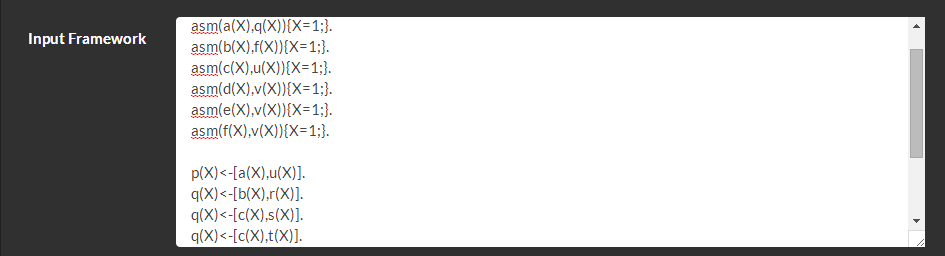
\includegraphics[width=0.8\textwidth]{argumentationText.png}
    \caption{Defining framework and targeted conclusion.}
    \label{fig:arg_text}
\end{figure}

The formal context free grammar of the input language along with how it is parsed is explained in detail in section [TODO].

\subsection{Configuration of the engines.}

Additionally the users should be able to choose the configuration of the derivation engine to be used. This includes two main decisions, the engine to be used and the semantics to be used.

The users can choose the engine required by checking the check-box as in example [TODO].

\begin{figure}[h]
    \centering
    
\includegraphics[width=0.8\textwidth]{argumentationEngines.png}
    \caption{Choosing derivation engine.}
    \label{fig:arg_engines}
\end{figure}

The user can then choose the semantics required by selecting the check-box corresponding to the required semantics, as in example [TODO].

\begin{figure}[h]
    \centering
    
\includegraphics[width=0.8\textwidth]{argumentationSemantics.png}
    \caption{Choosing semantics for derivation.}
    \label{fig:arg_semantics}
\end{figure}

[COULD INCLUDE JUST ONE IMAGE WITH ANNOTATION]

Lastly, the user must specify the claim for which a derivation is required as in example [TODO].

\begin{figure}[h]
    \centering
    
\includegraphics[width=0.8\textwidth]{argumentationConclusion.png}
    \caption{Declaring a targeted conclusion.}
    \label{fig:arg_conclusion}
\end{figure}

An example of the input form completed in its entirety can be seen at example [TODO]

\begin{figure}[h]
    \centering
    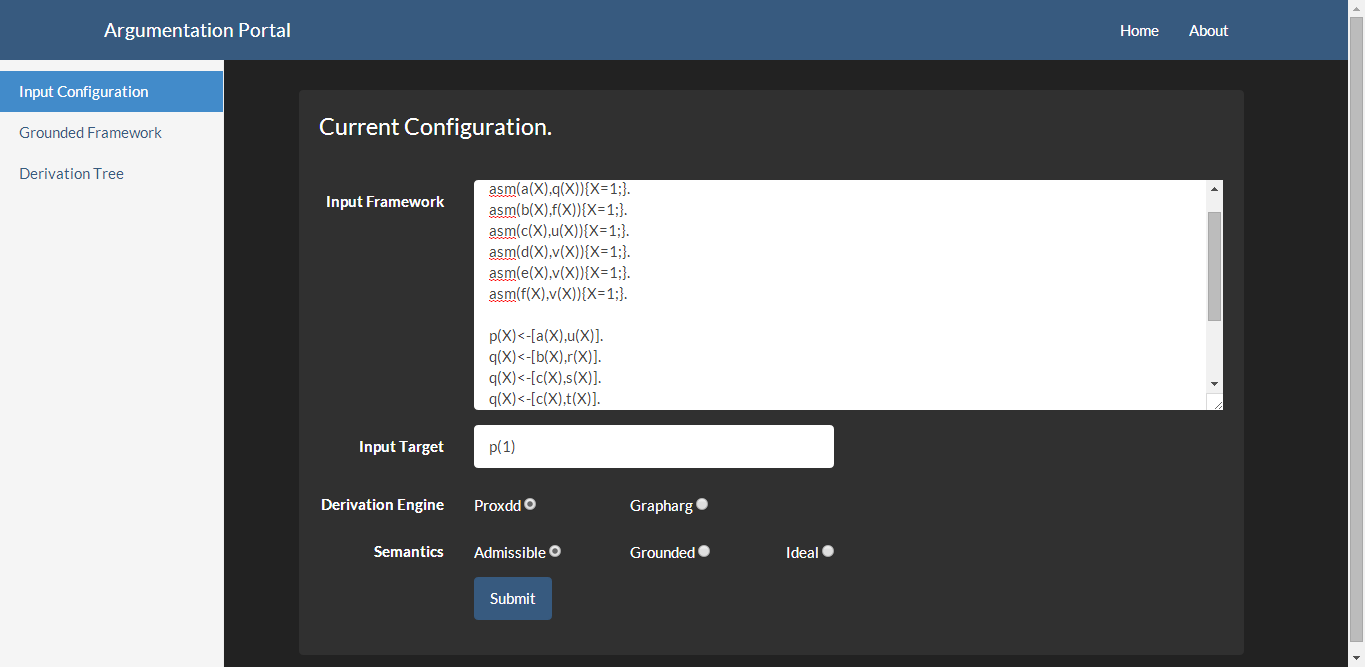
\includegraphics[width=0.8\textwidth]{argumentationInputFull.png}
    \caption{Example of completed input configuration form.}
    \label{fig:arg_input_full}
\end{figure}

\subsection{Visualisation the derivation tree.}

Once the input provided has been analysed by the derivation engines then the solution found is provided to the user as a derivation tree. Once the Server side finishes processing the solution it provides a JSON string that is interpreted client-side by javascript and the D3.js visualisation library. The JSON string has a structure as illustrated in example [TODO]. This structure specifies the characteristics of each node in the tree and the edges between the nodes.

\begin{Verbatim}[frame=single]
{ 
	"nodes":
	[
	{"id":"s0_0","name":"p(1)","shape":3,"group":0},
	{"id":"s0_1","name":"a(1)","shape":0,"group":1},
	]
	,"links":
	[
	{"source":1,"target":0,"value":1,"group":0},
	{"source":3,"target":2,"value":1,"group":0},
	{"source":2,"target":1,"value":1,"group":1},
	]
}
\end{Verbatim}

On the client side the JSON is processed and the derivation tree it represents is illustrated in the canvas area of the web page as shown in example [TODO]. The tree is annotated and colour coded for clarity and it also allows the user to zoom in and out.

\begin{figure}[h]
    \centering
    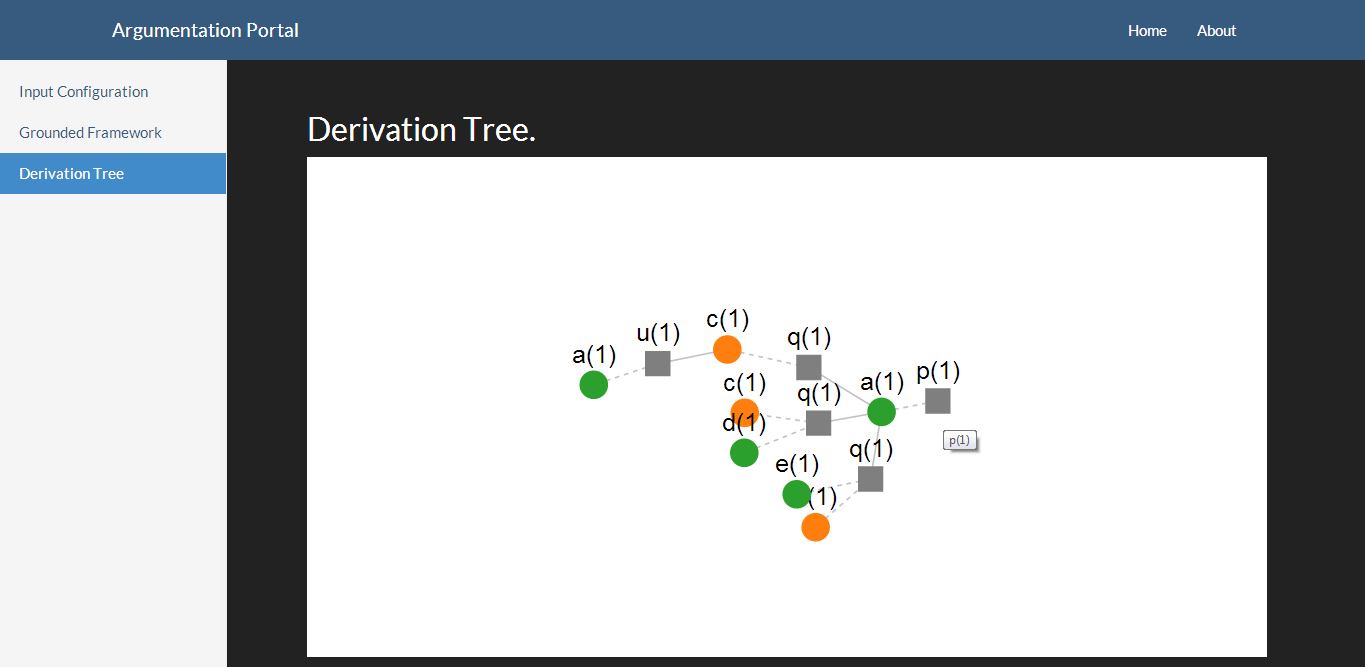
\includegraphics[width=0.8\textwidth]{argumentationTree.png}
    \caption{Visualisation of output as derivation tree.}
    \label{fig:arg_tree}
\end{figure}

\section{Server - Processing the Input.}

Once the user specifies the framework it then has to be passed to the server to be processed. Within the server several steps take place concerning the processing of the framework. These allow the interpretation of the input and the generation of the corresponding input for the engine. These steps include:

\begin{itemize*}
\item Parsing the Input and seperating the various elements (as described in [TODO]).
\item Checking the validity of the input (as described in [TODO]).
\item Grounding the input over a certain domaind (as desribed in [TODO]).
\item Generating the derivation engines input (as described in [TODO]).
\end{itemize*}

Due to the modularity of the web application it is possible that new derivation engines could be added to the back-end by implementing alternative to these steps. For example, if a new engine is added than by switching to a different generator we can now use the parsed and grounded input to create an input viable for the new derivation engine.

\section{Server - Interfacing with the Prolog Engine.}

Both Proxdd and Grapharg are implemented in the Prolog programming language which is commonly used in the field of AI. However, it has not been developed with web application development in mind which would hinder any attempts to extend the web application in the future if the whole of the server implementation was carried out in Prolog. 

\subsection{Need for an interface between C\# and Prolog Engines.}

The following decision choices were all possible:

\begin{itemize*}
\item Re-implementing both Proxdd and Grapharg in C\#
\item Using an external library that provides an interface for C\# with Prolog.
\item Implementing the back-end of the web application in Prolog.
\end{itemize*}

Nonetheless, for reasons explained in more detail in section [TODO] the use of an external library seemed to be the most reasonable choice. The interface allows for seamless integration of Prolog and C\#. Additionally, it enables us to focus most of the development work in a programming framework that is more popular and extendible than Prolog.

\subsection{Using the SwiPIC.dll library as an interface.}

The SwiPIC.dll library was chosen as it a provide a simple interface from C\# to the SWI-Prolog. It allows for the initialisation of an Instance of the SWI-Prolog Engine and we can then build Prolog queries that can be run. The code snippet at [TODO] provide an example of how the Prolog Engine is initialised and how a query is run:

\begin{Verbatim}[frame=single]

if (!PlEngine.IsInitialized)
{
    String[] param = { "-q", "-f", runProlog };  
    PlEngine.Initialize(param);

    using (PlQuery q = new PlQuery("loads(" + termList + "),
    		sxdd(" + claim.Text + ",X,Y)"))
    {
    	int idx = 0;
        foreach (PlQueryVariables v in q.SolutionVariables)
        {
        	solution.Add(v["Y"].ToString());
        }
    }
    PlEngine.PlCleanup();
}

\end{Verbatim}

By using an external library such as this we can easily interact with the derivation engines implemented in Prolog by submitting the query we have constructed based on the user's input and extracting the solution returned by the engine. The interface also enables us to implement the bulk of the application in C\# and then use external libraries such as this to interact with any other derivation engines in the future, while keeping the bulk of the implementation common.

\section{Choosing the current implementation.}

There are often enough more than one correct ways of designing and implementing a system. Related decisions are often taken based on the priorities of the project and other limitations. In this subsection I look into justifying some of the design decisions taken and potential disadvantages. Additionally we will look into one of the proposed alternatives for the derivation engines.

\subsection{Advantages of current implementation.}
The main advantage of the 3-tier system is that we provide modularity to the system allowing us to separate various significant elements of the system. In our implementation most of the processing other than the derivation is carried out in the Server tier by the C\# code. This makes it highly extendible as a simple switch can be implemented in the Server tier that enables the user to choose from an array of engines. The implementation, being modular, does not require extensive changes in the code to accommodate new derivation engines. As long as an interpreter is created to generate the required JSON string for the client side and the user input is translated to the correct corresponding input for the derivation engine, then the rest of the application should remain unchanged.

In addition to this the modular implementation allows the incorporation of further extensions to the application as part of the pre-processing process in the Server module. As an example, consider that there is a direct mapping that can be implemented between Abstract Argumentation and Assumption Based Argumentation. This mapping can be implemented in a module that is set to run as part of the pre-processing done in the Server module. This can be added to the process in a seamless manner, by which it can be enabled or disabled when required without any additional code changes.

Lastly, the choice to interact with the Prolog engine through an interface rather than the alternatives suggested was done for the purposes of usability and extensibility. Details of this approach are discussed in the last subsection [TODO]. 

\subsection{Disadvantages of current implementation.}

One of the disadvantages of the current implementation is its reliance on rather exotic external libraries to interface and run the Prolog derivation engines. There is the potential that if the web application is further developed in the future an updated version of this library might be required. However, as the library is not one of the core libraries in C\# such an update might take long to be released. Nonetheless, this was taken into account when deciding whether to used this library or not. The application deliberately tries to limit the use of this library to just initialising the engine, submitting a query and extracting the solution. The specifics of the query, for example, are built without the use of this library. Additionally, when deploying the application the environment needs to be configured to account for these libraries.

Another disadvantage of the current implementation is that there is currently a significant amount of processing required to generate the data communicated between the tiers in the required format. When a user inputs a framework this must then be translated in the required form for the input of the derivation engine. Once the derivation engine complete the solution then has to be interpreted and the corresponding JSON string must be generated. This takes processing time. An alternative would be to adapt the derivation engines to directly produce the JSON string rather than an alternative output. However, it would be unrealistic to expect derivation engines to conform to these standards. Instead, the current implementation allows for better integration of new engines rather than processing power.

\subsection{Proposed alternative (Prolog Web Server).}

There is one exceptionally interesting alternative implementation that was considered during the design process. SWI-Prolog which is the flavour of Prolog used in our implementation also provides the ability for it to run as a Web Server on its own. The proposed alternative is to establish a web server based on SWI-Prolog that would also include the derivation engines. This web server can then be configured to listen on certain ports for requests that it would be able to handle and reply to. Our web application would then be able to send over the required parameters of the derivation in the form of an Http Request to the Prolog Server. The Prolog Server would then carry out the derivation process and respond with the solution. A major potential advantage of this implementation would be that the Prolog Server could be used by further applications in the future. Requests can be made by various applications and these would be handled accordingly by the Prolog Server.

Nonetheless, there are issues that had to be considered when rejecting this alternative. Configuring the web server and the firewalls between it and our web application would be a very cumbersome task, which could be avoided. Also by creating a completely distinct web server to handle the derivation we are relying our web application on two servers. This creates two potential hazard points for our application. If the Prolog Web Server happens to stop working or face a fault then the web application will not work properly. By integrating Prolog through C\# we reduce this potential weakness point. Lastly, the idea of implementing the whole Server side of the application on a Prolog Web Server was rejected as Prolog is not a well supported web development framework such as C\# and ASP.Net. This would provide problems when having to extend the application to include new engines which might be built in other programming languages and frameworks such as C++, C, Pythonm etc.